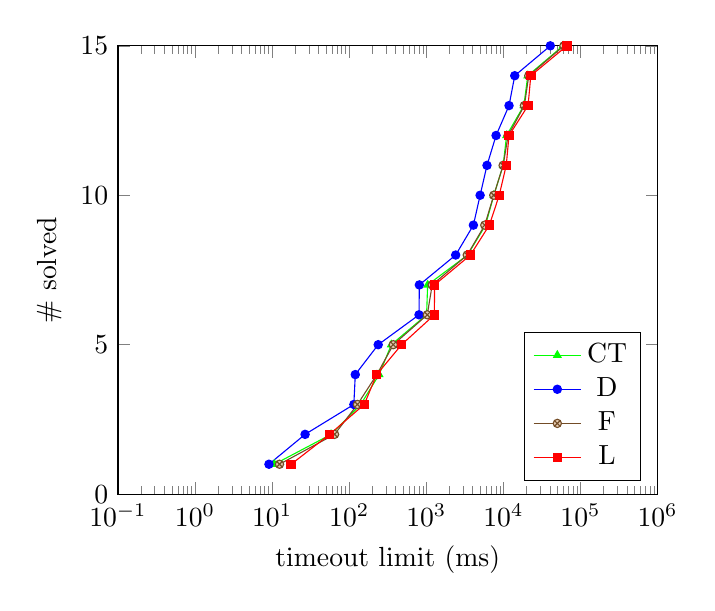
\begin{tikzpicture}[scale=1.0]
  \begin{axis}[
    xmode=log,
    ymin=0,ymax=15,
    xmin=0.1, xmax=1000000,
    every axis plot/.style={thin},
    xlabel={timeout limit (ms)},
    ylabel={\# solved},
    legend pos=south east
    % table/create on use/cumulative distribution/.style={
    %   create col/expr={\pgfmathaccuma + \thisrow{f(x)}}   
    % }
    ]
    \addplot 
    [mark=triangle*,
    mark size=1.5,
    mark options={solid},
    green] 
    coordinates {(10.724, 1)
(58.141, 2)
(140.926, 3)
(244.339, 4)
(351.655, 5)
(1007.846, 6)
(1040.618, 7)
(3429.804, 8)
(5862.337, 9)
(7518.829, 10)
(9922.216, 11)
(10995.644, 12)
(18421.925, 13)
(20703.909, 14)
(59350.857, 15)};

    \addplot 
    [blue,
    mark=*,
    mark size=1.5,
    mark options={solid}]
    coordinates {(9.092, 1)
(26.766, 2)
(114.809, 3)
(119.817, 4)
(237.752, 5)
(803.879, 6)
(812.209, 7)
(2403.255, 8)
(4081.014, 9)
(4986.668, 10)
(6124.842, 11)
(8030.718, 12)
(11828.045, 13)
(14031.517, 14)
(40586.867, 15)};

    \addplot [brown!60!black,
    mark options={fill=brown!40},
    mark=otimes*,
    mark size=1.5]
    coordinates {(12.465, 1)
(64.573, 2)
(127.898, 3)
(228.109, 4)
(372.722, 5)
(1029.302, 6)
(1191.482, 7)
(3392.266, 8)
(5728.998, 9)
(7496.585, 10)
(9916.094, 11)
(11510.717, 12)
(18700.846, 13)
(21320.804, 14)
(60889.133, 15)};

    \addplot 
    [red,
    mark size=1.5,
    mark=square*]
    coordinates {(17.667, 1)
(55.690, 2)
(156.556, 3)
(226.984, 4)
(477.676, 5)
(1271.053, 6)
(1280.040, 7)
(3730.514, 8)
(6571.512, 9)
(8823.766, 10)
(10881.983, 11)
(11821.394, 12)
(20882.392, 13)
(22667.922, 14)
(66608.065, 15)};
    \legend{CT,D,F,L}
  \end{axis}
\end{tikzpicture}
